\chapter{LQR Controller}
\label{section:lqr}

\section{Introduction}
\label{section:lqr introduction}

After validating the PID controller, the TA asked if it would be possible to design another controller able to only use
the second motor when the first one struggles to reach the desired speed. This desire suits to the system as the motor 2
is weaker than the first one: it can be seen easily as its time constant $\tau$ is greater than the one of motor 1, 
meaning that it needs more time to reach a set value.

\section{State Space Model}
\label{section:ss representation}
In control system design, it is often easier to define a parameterized state-space model in continuous time because 
physical laws are typically described using differential equations. The linear state-space representation in 
continuous-time has the following form:

\begin{equation}
    \dot{\mathbf{x}} = A \mathbf{x} + B \mathbf{u}
    \label{eq:state_space_models}
\end{equation}

where \( \mathbf{x} \) is the state vector, \( A \) is the state matrix that represents the system dynamics, 
\( B \) is the input matrix that represents the control input, and \( \mathbf{u} \) is the input vector.\\
To get to the state space representation from the transfer function is quite easy as each motor is a $1^{st}$ order
system. By using the following property of the Laplace transform:

\begin{align}
    X(s) &= \mathcal{L}\left\{x(t)\right\}\\
    s X(s) &= \mathcal{L}\left\{\frac{d x(t)}{dt}\right\}
\end{align}

The transfer function \ref{eq:1_st_order_TF} can be put in the temporal domain:

\begin{gather}
    G(s) = \frac{Y(s)}{U(s)} = \frac{A_0}{\tau s + 1}\\
    \left(\tau s + 1\right) Y(s) = A_0 U(s)\\
    \tau \dot{y}(t) + y(t) = A_0 u(t)\\
    \dot{y}(t) = \frac{-1}{\tau} y(t) + \frac{A_0}{\tau} u(t)
\end{gather}

This can be done for both motors with respectively ($u_1/y_1$) and ($u_2/y_2$) as input and output. With the choice of 
state $x_i(t) = y_i(t)$ representing the contribution of each motor to the total velocity, the state space 
representation becomes:

\begin{equation*}
    \dot{\mathbf{x}}(t) = \begin{bmatrix}
    \frac{-1}{\tau_1} & 0 \\ 
    0 & \frac{-1}{\tau_2}
    \end{bmatrix} \mathbf{x}(t) + \begin{bmatrix} 
    \frac{A_{01}}{\tau_1} & 0\\ 
    0 & \frac{A_{02}}{\tau_2} 
    \end{bmatrix}\mathbf{u}(t)
\end{equation*}

\begin{equation}
    y(t) = \begin{bmatrix} 1 & 1 \end{bmatrix}\mathbf{x}(t)
\end{equation}

where \( y \) is the velocity output, which is just the sum of both imposed speeds ($y = y_1 + y_2$). It is however 
known that the states are not really independent so this state space representation is not accurate.the following 
simplified model will be used from now where the state is a single value, namely the velocity of the shaft.

\begin{equation}
    \dot{\mathbf{x}}(t) = \begin{bmatrix}-\frac{\tau_1+\tau_2}{2 \tau_1 \tau_2}\end{bmatrix} \mathbf{x}(t) + 
    \begin{bmatrix} 
     \frac{A_{01}}{\tau_1} & \frac{A_{02}}{\tau_2} 
    \end{bmatrix}\mathbf{u}(t)
    \label{eq:state_space_model_cx}
\end{equation}

\begin{equation}
    y(t) = \mathbf{x}(t)
    \label{eq:state_space_model_cy}
\end{equation}

\section{Discrete-Time State-Space Model}
We need to convert the continuous-time state-space model \eqref{eq:state_space_model_cx} and 
\eqref{eq:state_space_model_cy} to a discrete-time state-space model to design the controller in discrete time. This is
the other approach compared to the one used in section \ref{section:PID controller} as we were there building the 
controller in continuous time and then we discretized it. Using the parameters from the identification 
section (\ref{section:identification}):

\[
\tau_1 = 1.915, \quad \tau_2 = 1.7, \quad A_{01} = 24.88, \quad A_{02} = 19.51
\]

The continuous-time matrices are computed:

\[
\mathbf{A} = 
\begin{bmatrix}
-0.5552
\end{bmatrix}, \quad 
\mathbf{B} = 
\begin{bmatrix}
12.9870 & 11.4765
\end{bmatrix}.
\]

For a sampling time \( T_s = 0.005 \, \text{seconds} \), the discrete-time matrices \( A_{T_s} \) and \( B_{T_s} \) are calculated as follows:

\begin{itemize}
    \item \textbf{Discrete-Time State Matrix} (\(A_{T_s}\)): 
   Using the matrix exponential formula:
   \begin{gather*}
        A_{T_s} = e^{A T_s} = \begin{bmatrix} 1.0028 \end{bmatrix}    
   \end{gather*}
   

\end{itemize}


\begin{itemize} 
    \item \textbf{Discrete-Time Input Matrix} (\(B_{T_s}\)): 
   Using the formula:
   \begin{gather*}
    B_{T_s} = \int_0^{T_s} e^{A \zeta} B \, d\zeta = \begin{bmatrix} 0.0648 & 0.0573\end{bmatrix}    
   \end{gather*}
   
\end{itemize}

Thus, the discrete-time state-space representation of the system is:

\begin{gather*}
    \mathbf{x}[k+1] = 
        \begin{bmatrix} 1.0028 \end{bmatrix} \mathbf{x}[k] 
    + \begin{bmatrix} 0.0648 & 0.0573 \end{bmatrix} \mathbf{u}[k]\\
    \mathbf{y}[k] = \mathbf{x}[k]
\end{gather*}


Finally, the sampled system is equivalent to a discrete-time system with these matrices. We will now use this representation to design an LQR controller for the given discrete-time system.

\section{Controller design}

\subsection{Simple state feedback}

In the case of this system and because the model has been simplified to a single state representation in section
\ref{section:ss representation}, there is no need to build an observer as the state is the velocity measured by the 
speed sensor. This gives rise to a really simple block diagram:

\begin{figure}[H]
    \centering
    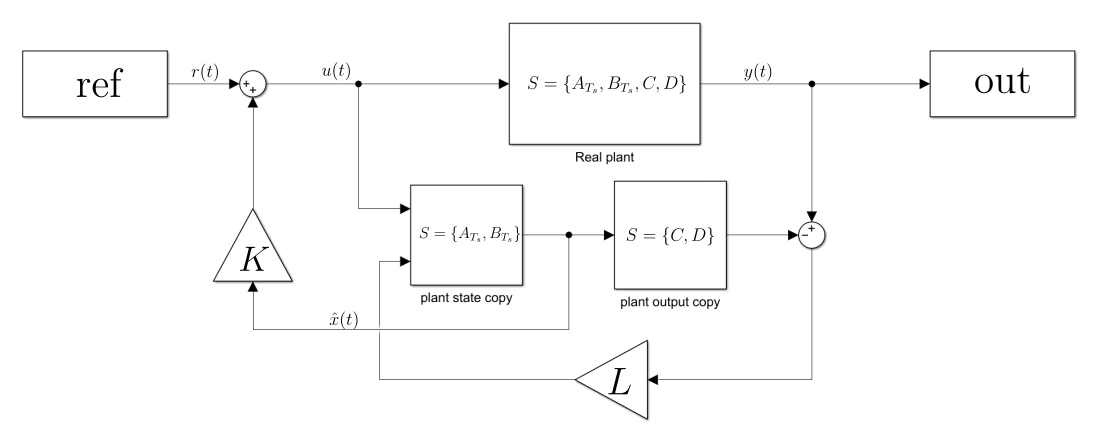
\includegraphics[width = \textwidth]{Pictures/lqr_controller.png}
    \caption{Structure of the LQR controller}
    \label{fig:lqr structure}
\end{figure}

The determination of the value for $K$ has been done using the LQR algorithm.
% observer derivation, left in comment with respect to the time spent writing the subsection :')

\iffalse
\subsection{Observer}

The observer will consist of a copy of the system and a feedback as shown in fig \ref{fig:observer structure}. In this
section, the matrix $L$ must be determined in a way such that the resulting observer is asymptotic.

\begin{figure}[H]
    \centering
    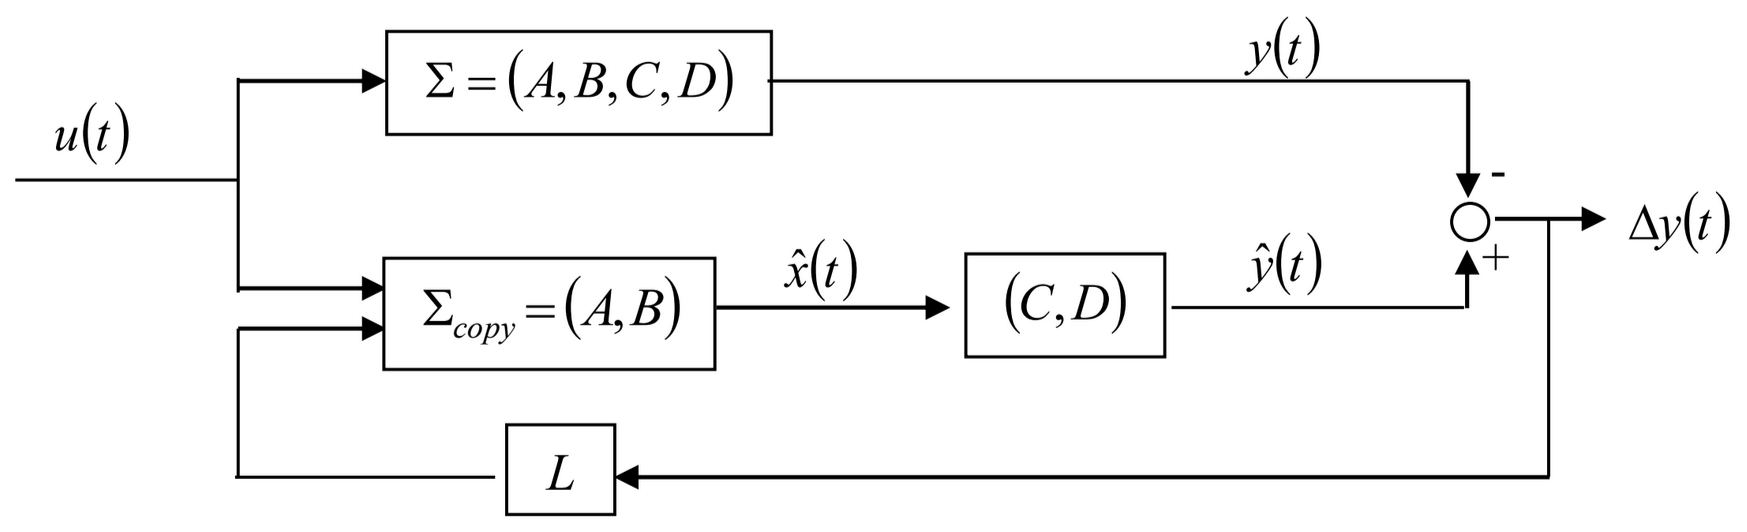
\includegraphics[height=\textheight/7]{Pictures/observer_general_structure.png}
    \caption{Generic structure of an observer}
    \label{fig:observer structure}
\end{figure}

For an observer to be asymptotic, the eigenvalues of $(A + LC)$ must be converging. It is however important to not skip
a step in the design. First, the observability matrix $\mathcal{O}_2$ of the system must be computed:

\begin{equation}
    \mathcal{O}_2 = 
    \begin{bmatrix}
        C\\
        C A_{T_s}
    \end{bmatrix}
    =
    \begin{bmatrix}
        1 & 1\\
        0.9974 & 0.9971
    \end{bmatrix}
\end{equation}

Now that we are sure that $\mathcal{O}_2$ is full rank, we can conclude that the system is detectable and that a matrix
L that will make the observer asymptotic exists. Because the state error $\hat{x}(t) - x(t)$ converges with 
$\lambda_i^t$\footnote{$\lambda_1$ and $\lambda_2$ being the eigenvalues of $A_{T_s} + LC$}, it is a smart choice to try to make
those $\lambda_i$ close to 0.

\begin{gather}
    L = \begin{bmatrix} l_1\\l_2 \end{bmatrix}\\
    A_{T_s} + L C = \begin{bmatrix} 1+l_1 & 1+l_2 \\ 0.9974+l_1 & 0.9971+l_2 \end{bmatrix}
\end{gather}

An easy choice is $l_1 = -0.9974$ and $l_2 = -1$ to make $A_{T_s} + LC$ diagonal while ensuring that $\left|\lambda_i
\right| < 1$. This gives the final L matrix:

\begin{equation}
    L = \begin{bmatrix}
        -0.9974 \\ -1
    \end{bmatrix}
\end{equation}
\fi

The goal of the Linear Quadratic Regulator (LQR) is to minimize the quadratic cost function:

\[
J = \sum_{k=0}^\infty \left( x[k]^\top Q x[k] + u[k]^\top R u[k] \right).
\]

Where the weighting square matrices \( Q \) and \( R \) must be selected based on system requirements:

\begin{itemize}
    \item \( Q \): Penalizes state deviations
    \item \( R \): Penalizes large control efforts
\end{itemize}

Because we have a single state, $Q$ will have no impact. The interesting parameter to play with is the matrix $R$ as the
value on its diagonal will determine the "\textit{cost}" of each input. The following choice has been made because, as 
said in the introduction \ref{section:lqr introduction}, we want to use the second motor only when the first one cannot 
produce enough torque:

\[
Q = 1, \quad
R = \begin{bmatrix}
1 & 0 \\
0 & 5
\end{bmatrix}.
\]

We then computed the feedback matrix using the matlab function \texttt{dlqr}:

\[
K = \begin{bmatrix}
    -0.0368\\
    -0.0065
\end{bmatrix}
\]

Finally, the step response of the system with a state feedback has been measured (fig \ref{fig:state feedback step 
response}). We can conclude from the data below that with a properly designed state feedback, the controller can mainly
use the $1^{st}$ motor and only send an input to the second motor when the reference is hard to reach (e.g. the step).
However this is far from satisfying us as there is  a steady state error. In the next section, we'll explain how to get 
rid of it.

\begin{figure}[H]
    \centering
    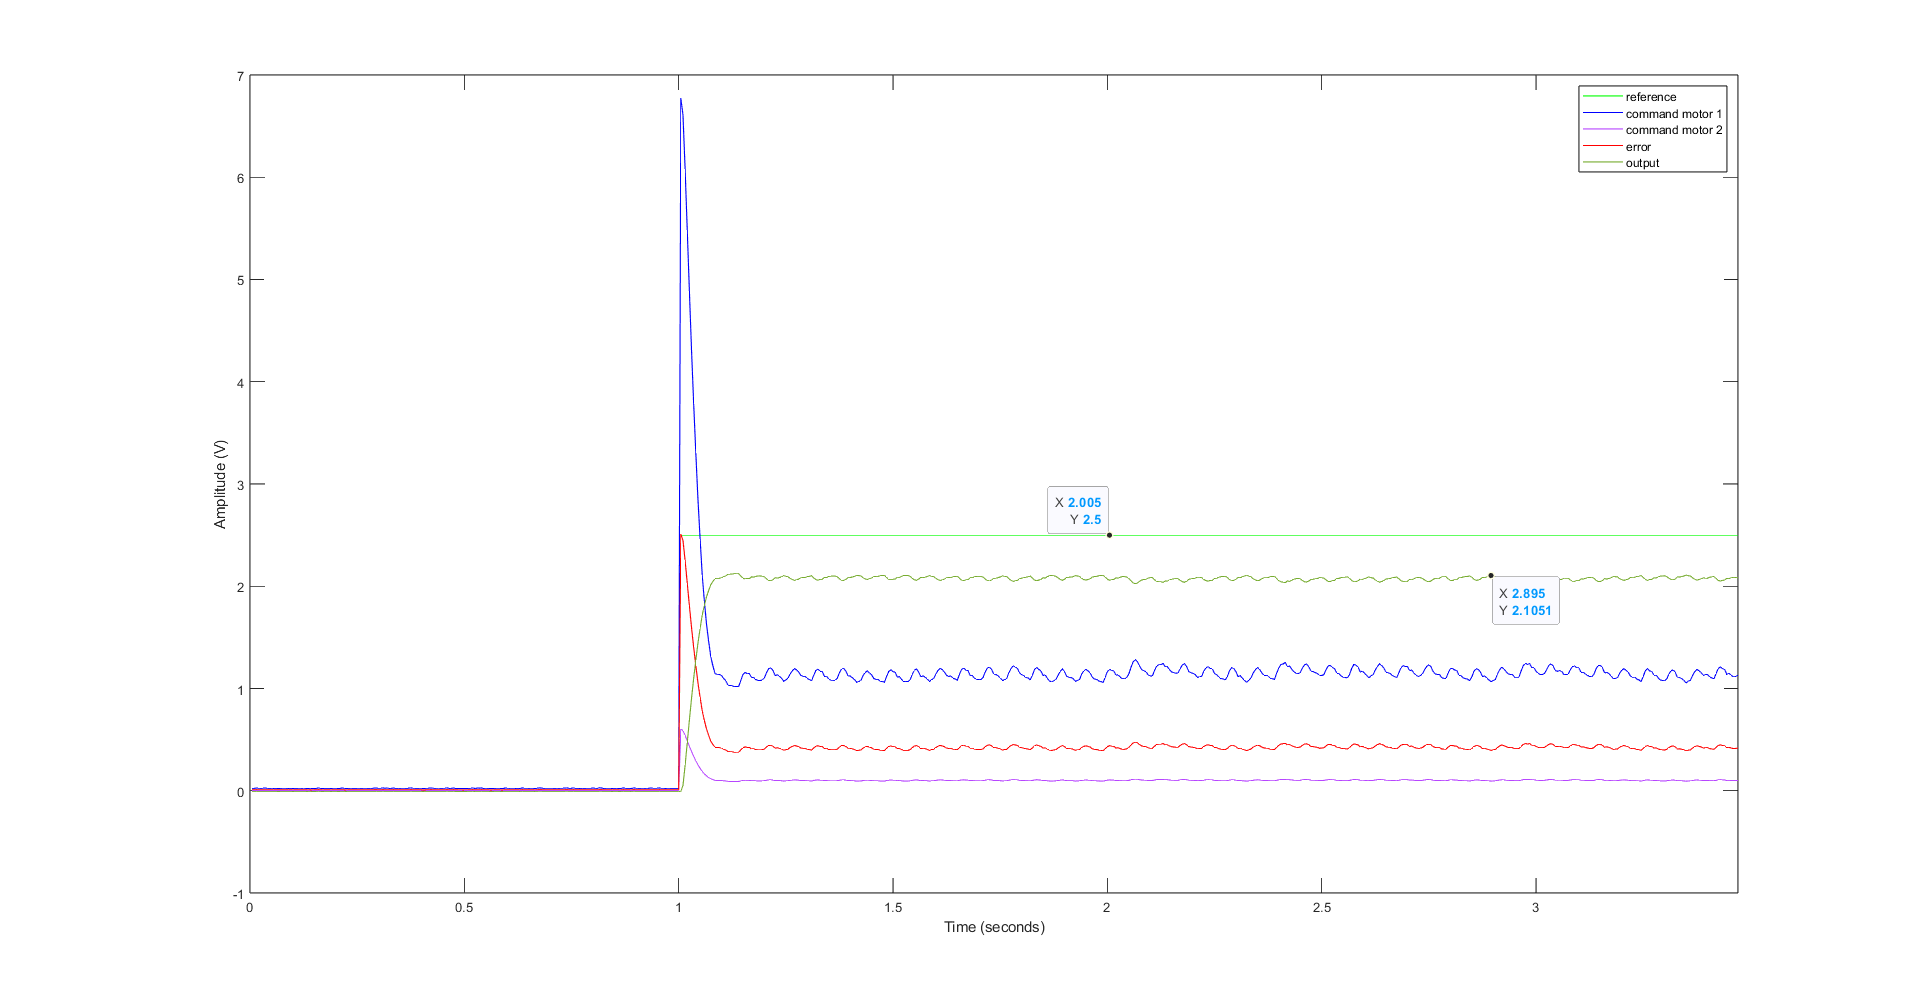
\includegraphics[width = \textwidth]{Pictures/without_PI.png}
    \caption{Step response with a state feedback}
    \label{fig:state feedback step response}
\end{figure}

\subsection{state feedback with an integrator}

To ensure a zero steady-state error, the closed loop system must contain a pole at the origin. This can be very easily 
done by adding an integrator in front of the feedback. However, the matlab documentation gives a function specifically
designed for an LQR state feedback with an integrator: \texttt{lqi}.

\begin{figure}[H]
    \centering
    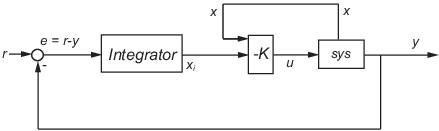
\includegraphics[width = \textwidth]{Pictures/lqi_docs.png}
    \caption{LQI structure, from matlab documentation}
    \label{fig:lqi documentation}
\end{figure}

This structure implies that $K$ becomes a $2x2$ matrix because its input is now the state $x$ and the output of the 
integrator $x_i$. The integrator has been discretized using the Tustin equivalence and the new K has been computed using
the same $R$ matrix than before. After trying with $Q = 1$, it has been increased to reduce the settling time which gave
the second graph.

\begin{figure}[H]
    \centering
    % Left Image
    \begin{subfigure}[b]{0.5\textwidth}
        \centering
        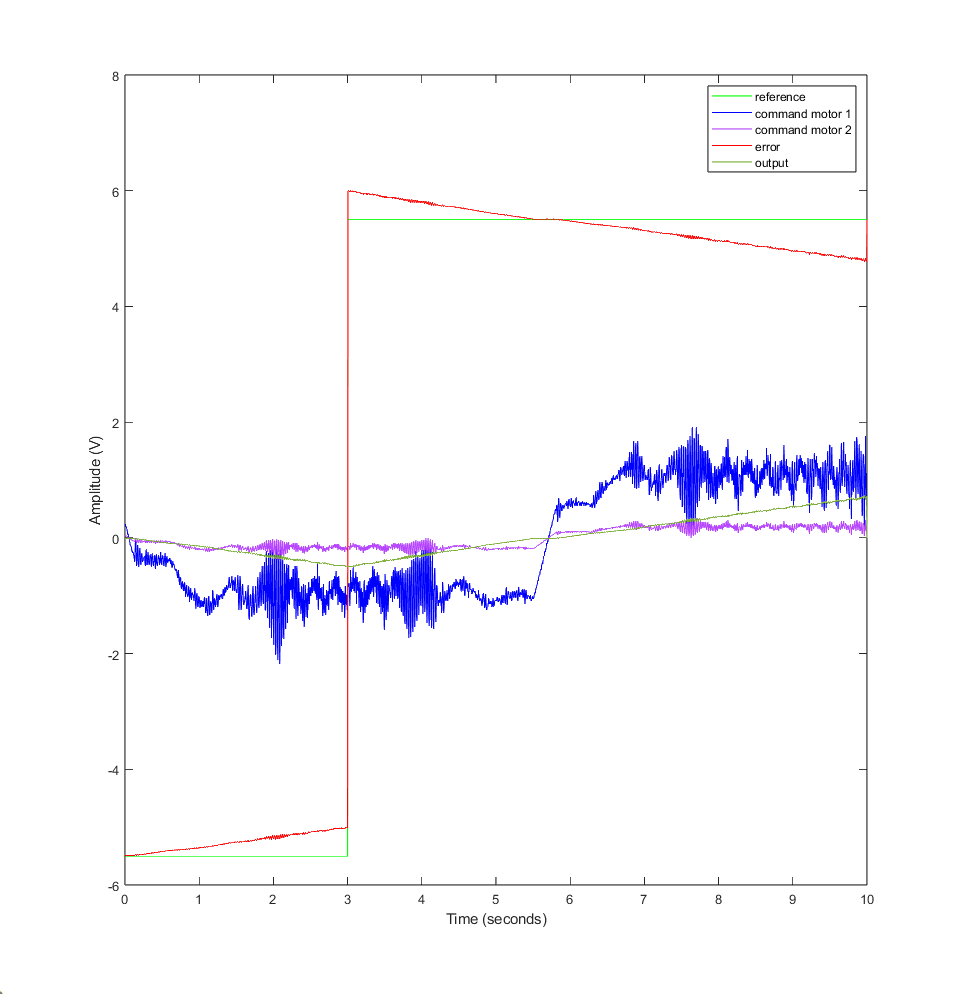
\includegraphics[width=\textwidth]{Pictures/Q_1.png}
        \caption{Step response of the LQI with $Q = 1$}
        \label{fig:step_response_Q1}
    \end{subfigure}%
    % Right Image
    \begin{subfigure}[b]{0.5\textwidth}
        \centering
        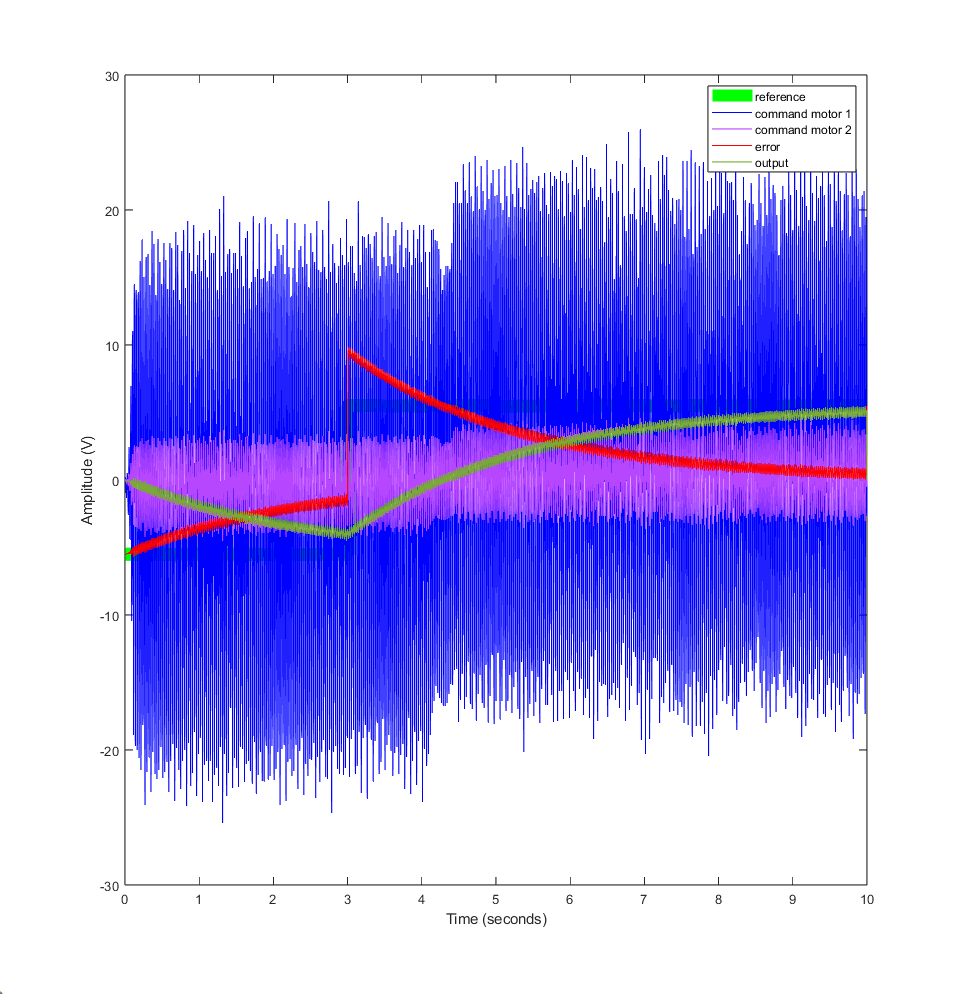
\includegraphics[width=\textwidth]{Pictures/Q_500.png}
        \caption{Step response of the LQI with $Q = 500$}
        \label{fig:step_response_Q500}
    \end{subfigure}
    \caption{Comparison of step responses for different $Q$ values}
    \label{fig:step_responses}
\end{figure}

Increasing $Q$ indeed helped to make the system reach the reference faster but it comes with an increase in the command
swing. A way to make it a better was to express $Q$ as a $2x2$ matrix. Let's recall from the previous section that $Q$
penalizes state deviation and because of the integrator, the state has become $\begin{bmatrix}y(t) & x_i(t)\end{bmatrix}
^T$ which means that only the integrator state (which controls the settling time) could be increased.

\begin{equation*}
    Q = \begin{bmatrix}
        \frac{1}{100} & 0\\
        0 & 100
    \end{bmatrix}
\end{equation*}

Allowed indeed a settling time close to the one of $Q = 500$ shown above (\ref{fig:step_response_Q1}) with
less input fluctuations. The best way found was in fact to let $Q = 1$ and to give more impact to the integrator by
adding a multiplier block $K_i$ at its output, giving the control scheme:

\begin{figure}[H]
    \centering
    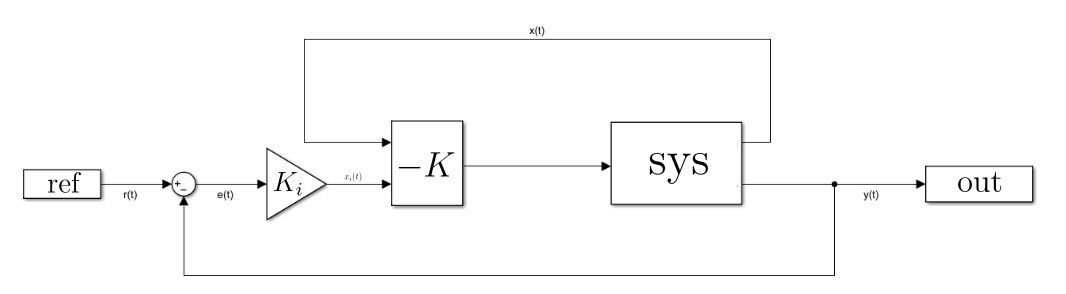
\includegraphics[width = \textwidth]{Pictures/lqi_controller.png}
    \caption{LQI adapted structure}
    \label{fig:lqi modified}
\end{figure}

Here again, two experiments have been made. The one on the left is with a low $K_i$ ($= 50$) and $R = 
\begin{bmatrix}1&0\\0&10\end{bmatrix}$ where the second test was conducted with $K_i = 500$ and $R$ has been set to
$\begin{bmatrix}1&0\\0&20\end{bmatrix}$.

\begin{figure}[H]
    \centering
    % Left Image
    \begin{subfigure}[b]{0.5\textwidth}
        \centering
        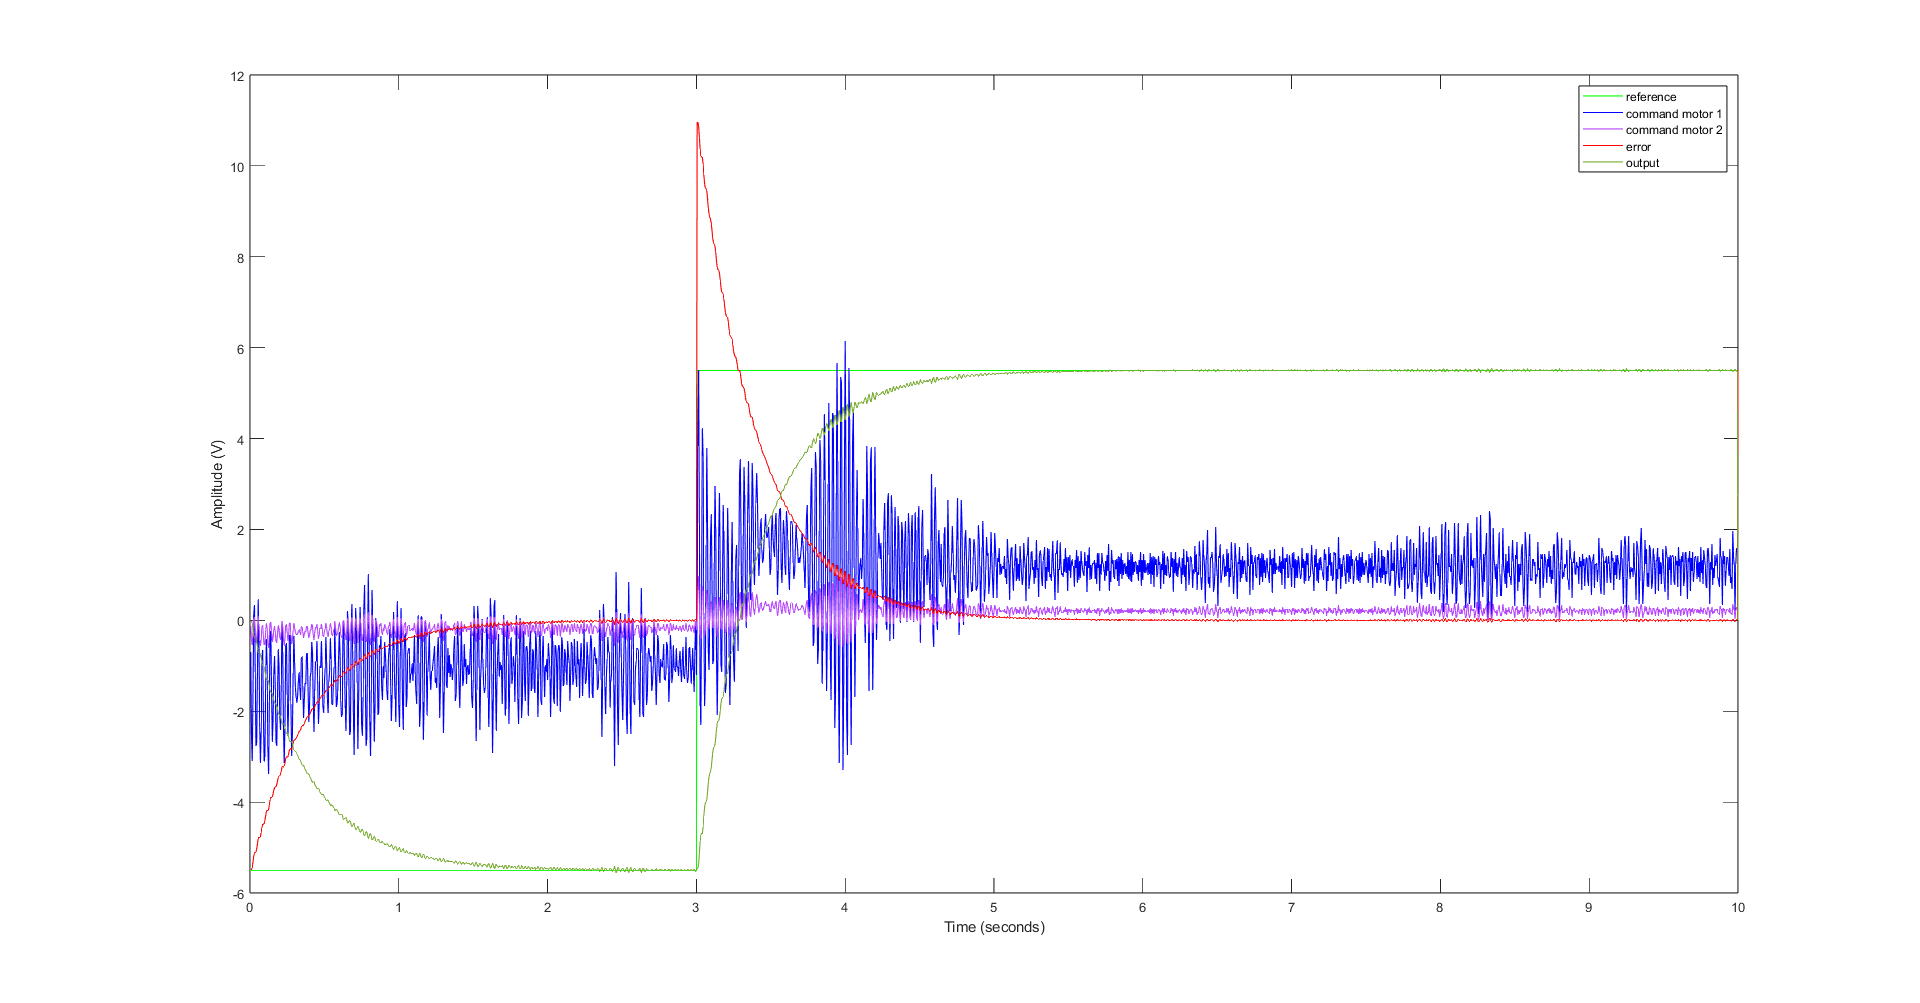
\includegraphics[width=\textwidth]{Pictures/McGiver1.png}
        \caption{Step response of the LQI with low $K_i$}
    \end{subfigure}%
    % Right Image
    \begin{subfigure}[b]{0.5\textwidth}
        \centering
        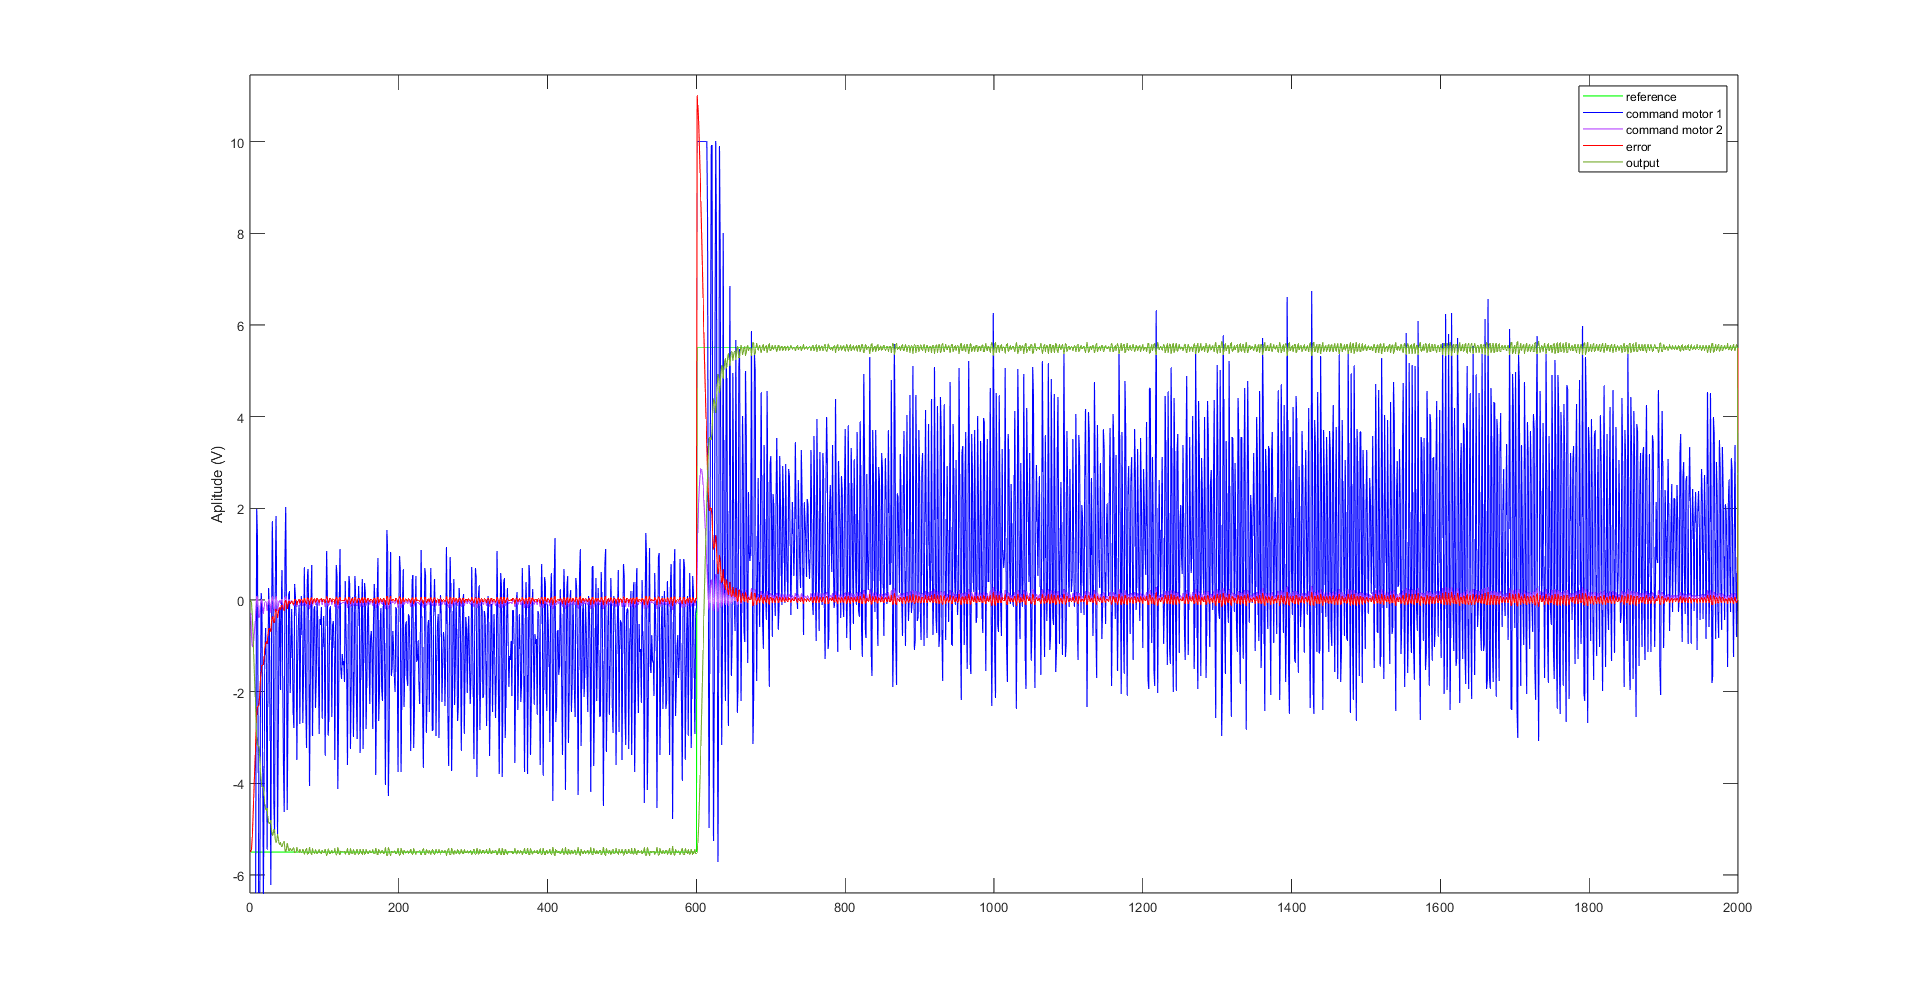
\includegraphics[width=\textwidth]{Pictures/McGiver2.png}
        \caption{Step response of the LQI with high $K_i$}
    \end{subfigure}
    \caption{Comparison of step responses for different $K_i$ values}
\end{figure}

The second one satisfying the settling time requirement, it has been chosen as the final LQI controller. A closer look
at the step (done in figure \ref{fig:lqi zoom}) shows that the second motor is indeed used when the $1^{st}$ motor is
not able to provide enough torque by itself (when a step reference is applied).\\
Due to the limited time we had in the lab, we were not able to conduct a disturbance test on this controller but as it
contains an integrator, it is (\textit{at least theoretically}) able to reject a step disturbance. The same thing applies
for the frequency response where the limited time only allowed us to manually measure the amplitude and the phase of the
closed loop at $4 Hz$ thanks to figure \ref{fig:lqi 4Hz}.

\begin{gather*}
    \text{Amplitude}\Big|_{f = 4 Hz} \simeq \frac{2.858}{4.99} = -4.84 dB\\
    \text{Phase}\Big|_{f = 4 Hz} \simeq \frac{0.315 - 0.355}{0.25} = -57.6^{\circ}
\end{gather*}

So we are definitely not achieving the $4^{th}$ requirement which was to perfectly track a $4 Hz$ signal.

\begin{figure}[H]
    \centering
    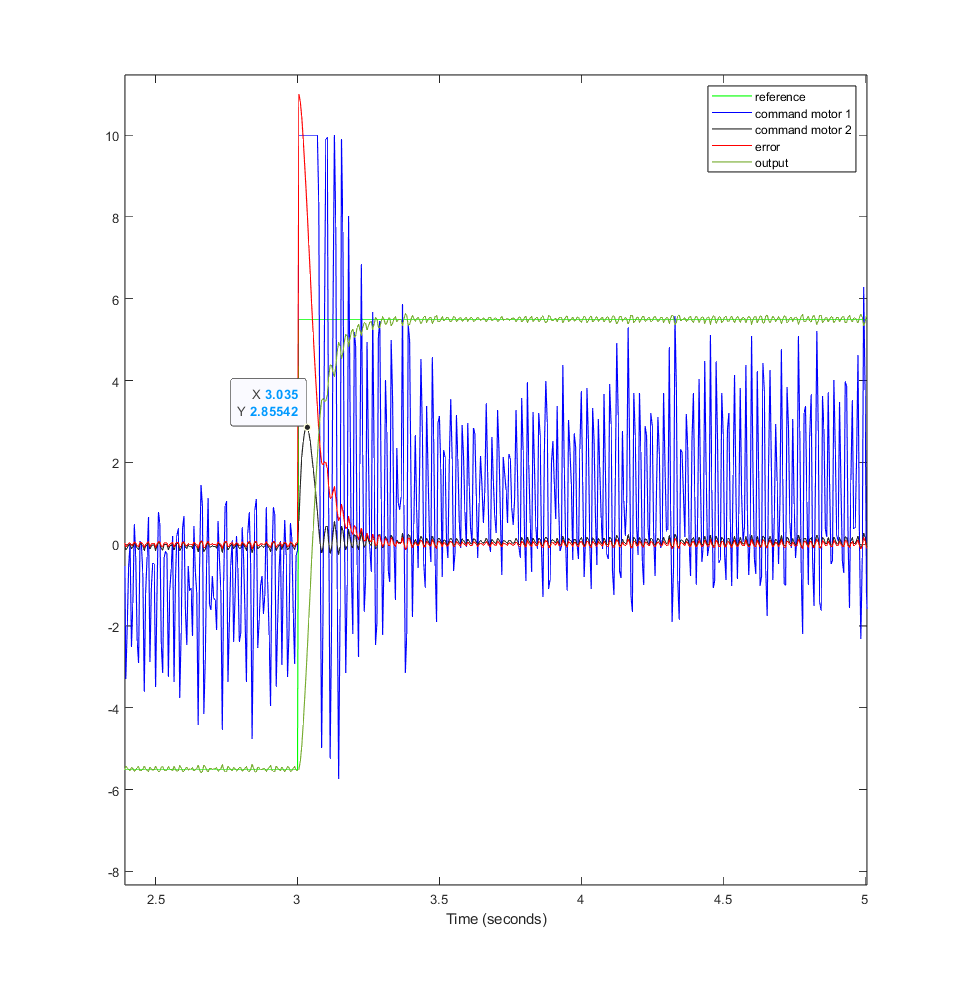
\includegraphics[width = \textwidth]{Pictures/McGiver_zoom.png}
    \caption{closer look to the step response of the final LQI controller}
    \label{fig:lqi zoom}
\end{figure}

\begin{figure}[H]
    \centering
    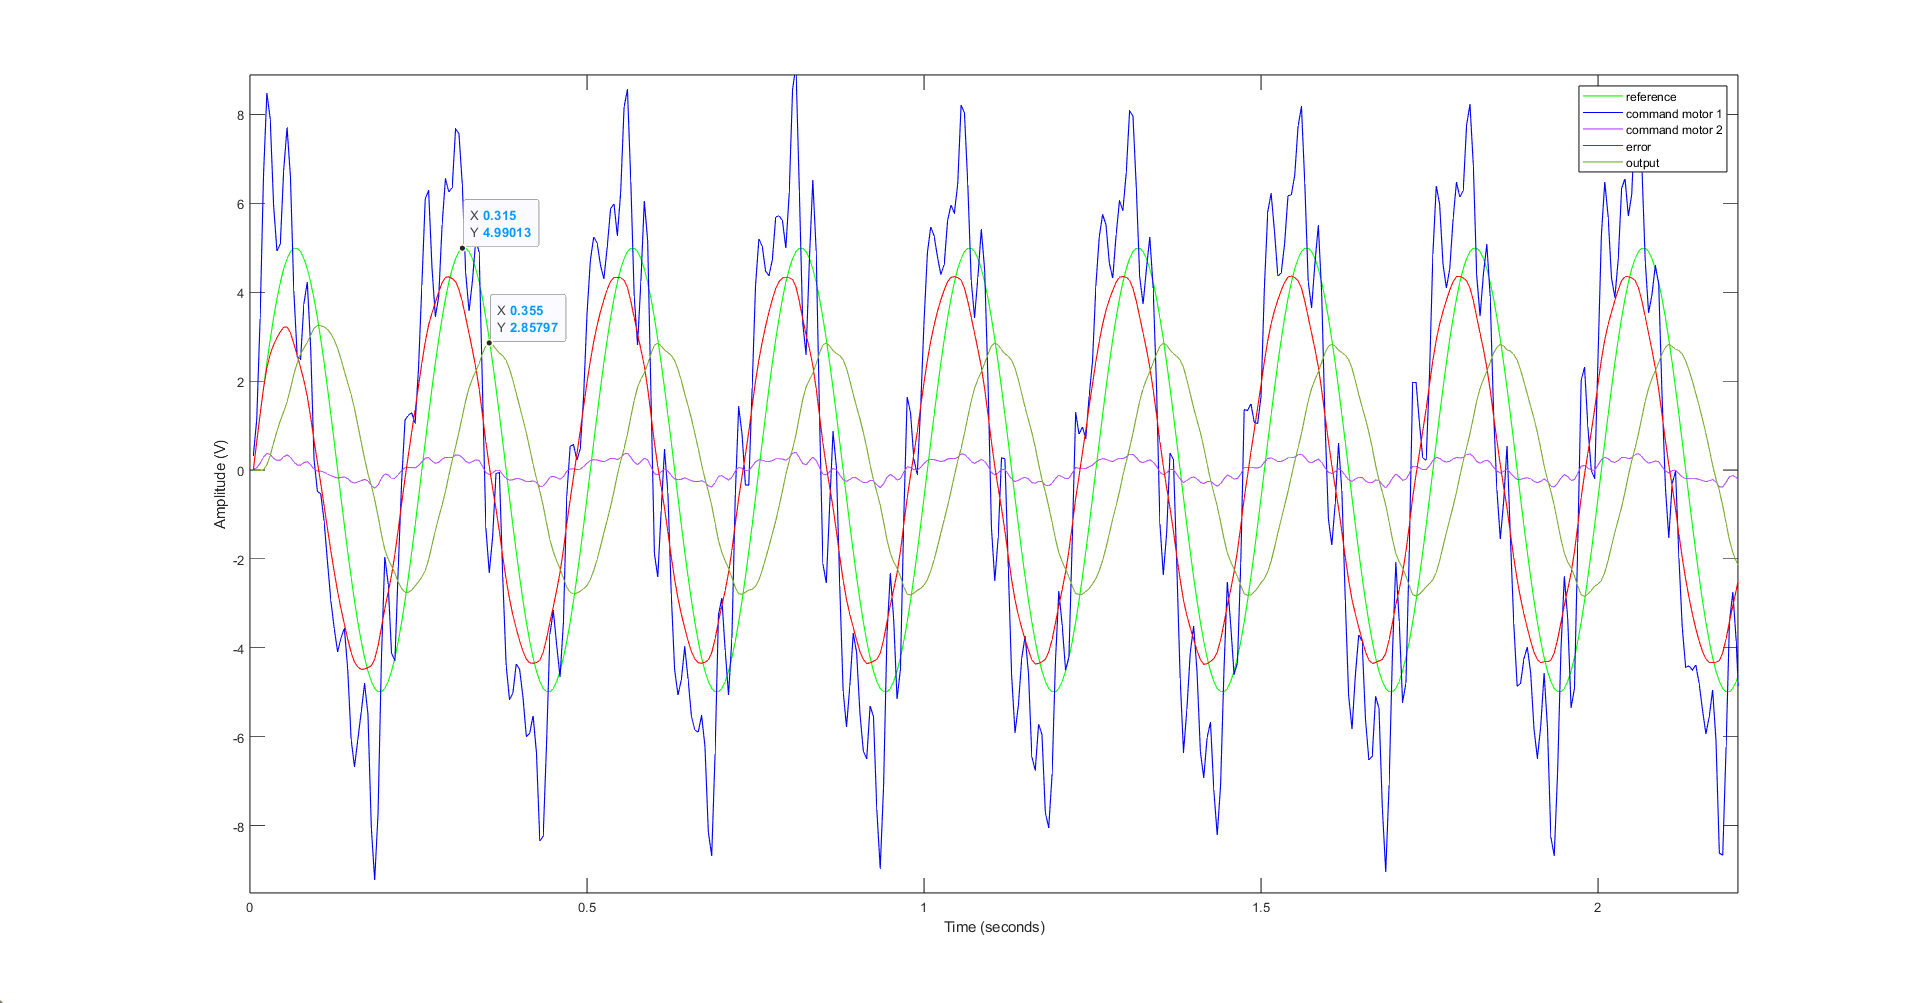
\includegraphics[width = \textwidth]{Pictures/frequency_response.png}
    \caption{Response of the final LQI controller to a $4 Hz$ sine reference}
    \label{fig:lqi 4Hz}
\end{figure}


